\documentclass[titlepage,11pt]{article}
\usepackage{comment}
\usepackage{enumitem}
\usepackage{listings}
\usepackage{amsmath}
\usepackage{graphicx}
\usepackage[font=small,labelfont=bf]{caption}
\usepackage[bahasa]{babel}
\usepackage{float}
\usepackage{verbatim}
\usepackage{graphicx,tabularx,multirow}
\usepackage{xcolor}
\usepackage{indentfirst}
\usepackage{subcaption}
\usepackage{pifont}
\usepackage[onehalfspacing]{setspace}
\usepackage[
	allcolors=visigrey,
	colorlinks=true,
]{hyperref}
\usepackage[a4paper,left=2cm,right=2cm]{geometry}
% Pengaturan kutipan artikel
\usepackage[style=ieee, backend=biber]{biblatex}
%Code listing style pak akok
\definecolor{codegreen}{rgb}{0,0.6,0}
\definecolor{codegray}{rgb}{0.5,0.5,0.5}
\definecolor{codepurple}{rgb}{0.58,0,0.82}
\definecolor{backcolour}{rgb}{0.95,0.95,0.92}

\lstdefinestyle{mystyle}{
	backgroundcolor=\color{backcolour}, commentstyle=\color{codegreen},
	keywordstyle=\color{magenta},
	numberstyle=\small\color{codegray},
	stringstyle=\color{codepurple},
	basicstyle=\ttfamily\footnotesize,
	breakatwhitespace=false,         
	breaklines=true,                 
	captionpos=t,                    
	keepspaces=true,                 
	numbers=left,                    
	numbersep=5pt,                  
	showspaces=false,                
	showstringspaces=false,
	showtabs=false,           
	frame = single,
	tabsize=2
}
\lstset{style=mystyle}

\definecolor{visigrey}{rgb}{.1,.15,.15}
\geometry{top=1cm,bottom=.5cm}
\savegeometry{titlepage}
\geometry{top=2cm,bottom=2cm}
\savegeometry{main}

\def\bspace{\(\qquad\qquad\qquad\)}
\usepackage[T1]{fontenc}
\usepackage[utf8]{inputenc}
\usepackage{tgheros}
\renewcommand*\familydefault{\sfdefault}

\setcounter{tocdepth}{6}

\def\autor{Laboratorium }
\def\lab{Multimedia dan Internet of Things}
\def\departemen{Departemen Teknik Komputer}
\def\institut{Institut Teknologi Sepuluh Nopember}
\def\praktikum{Praktikum \\ Jaringan Komputer}
\def\nama{Cedric Anthony Edysa - 5024221015 \\ Larasati Lituhayu - 5024221025 \\ Azaria Putri Fawnia - 5024221038\\Vania Bunga Febrina - 5024221069}
% Ubah Judul sesuai dengan modul
\def\judul{Mengelola dan Membagi Bandwith menggunakan Qos (Simple Queue)}
\def\tanggal{2024}
\begin{document}
% Ubah Bahasa sesuai dengan keinginan
\selectlanguage{bahasa}

\def\headingtype{\bf \small}
\loadgeometry{titlepage}
\begin{titlepage}
	\centering
	\begin{tabularx}{\textwidth}{Xr}
		\multirow[c]{6}{*}{
\includegraphics[width=3cm]{Cover/img/logodepart.png}} & {\emph{\headingtype \autor}}    \\ [-2pt]
		                                                                          & {\headingtype \lab}             \\[-2pt]
		                                                                          & {\headingtype \departemen}      \\[-2pt]
		                                                                          & {\headingtype \emph{\institut}} \\[-2pt]
		\vspace{1.6cm}
	\end{tabularx}\par
	\vspace{5.0cm}
	{\Huge \bf  \praktikum \par}
	\vspace{2.0cm}
	{\LARGE \bf \judul \par}
	\vspace{2.0cm}
	{\Large \nama \par}
	\vfill
	{\Large \tanggal \par}
	\vfill
	{\centering
		
\includegraphics[width=\textwidth]{Cover/img/footer.png}
	}
\end{titlepage}
\loadgeometry{main}
% Pilih Modul yang akan di build
\section{Pendahuluan}
\indent Manajemen bandwidth adalah suatu pendekatan yang digunakan untuk mengatur dan mengontrol
penggunaan bandwidth dalam suatu jaringan komputer. Dalam jaringan yang sibuk, alokasi bandwidth yang efisien dan adil sangat penting untuk menjaga kinerja jaringan yang optimal. Salah satu cara
untuk mengimplementasikan manajemen bandwidth adalah dengan menggunakan QoS atau Quality
of Service.
\\ \indent Quality of Service (QoS) adalah konsep yang digunakan dalam jaringan komputer untuk mengatur dan memberikan prioritas terhadap jenis-jenis data yang berbeda. Dengan menerapkan QoS,
administrator jaringan dapat mengatur penggunaan bandwidth, latency, jitter, dan keandalan layanan
dalam jaringan. QoS memungkinkan pengaturan prioritas, pembatasan bandwidth, dan penjadwalan
yang lebih baik untuk aplikasi atau protokol tertentu.
\\ \indent Dalam lingkungan jaringan yang padat, sering kali beberapa pengguna menggunakan aplikasi atau
protokol yang mengkonsumsi bandwidth yang tinggi, seperti video streaming atau file sharing, sementara pengguna lainnya mungkin hanya perlu menggunakan aplikasi yang membutuhkan bandwidth yang lebih rendah, seperti browsing web atau email. Tanpa manajemen bandwidth yang efektif,
pengguna dengan aplikasi berat bisa mendominasi sebagian besar bandwidth, menyebabkan kualitas layanan yang buruk bagi pengguna lain. Simple Queue adalah salah satu metode manajemen
bandwidth yang umum digunakan dalam router atau perangkat jaringan untuk mengatasi masalah ini.
\\ \indent Dalam Simple Queue, bandwidth diatur dengan membuat aturan atau kebijakan yang mendefinisikan
sejumlah parameter, seperti kapasitas maksimum bandwidth yang dapat digunakan oleh pengguna,
prioritas, dan pembatasan lainnya. Setiap paket data yang melewati router akan dicek dan diberi label sesuai dengan aturan tersebut, dan kemudian akan dikirim atau ditunda sesuai dengan prioritas
dan alokasi bandwidth yang ditentukan. Dengan menggunakan Simple Queue, administrator jaringan
dapat memastikan bahwa penggunaan bandwidth dijaga secara adil dan efisien. Pengguna dengan
kebutuhan bandwidth yang tinggi dapat diberikan alokasi yang lebih besar, sementara pengguna dengan kebutuhan yang lebih rendah tidak akan terpengaruh oleh penggunaan yang berlebihan. Hal
ini membantu memastikan kualitas layanan yang lebih baik bagi seluruh pengguna dalam jaringan.
Selain itu, Simple Queue juga memungkinkan administrator jaringan untuk memprioritaskan jenis lalu
lintas tertentu, misalnya memberikan prioritas lebih tinggi untuk aplikasi bisnis daripada aplikasi hiburan. Dengan demikian, manajemen bandwidth dengan Simple Queue dapat membantu meningkatkan
efisiensi penggunaan bandwidth, mengoptimalkan kinerja jaringan, dan menghindari situasi di mana
penggunaan bandwidth yang tidak adil atau berlebihan mengganggu pengalaman pengguna lainnya.

%===========================================================%

\section{Tujuan Praktikum}
Mengetahui cara melimitasi dan memanagemen bandwith untuk suatu jaringan yang banyak pengguna serta dapat memahami pengonfigurasian terkait Bandwith menggunakan Qos (Simple Queue)
%===========================================================%

\section{Alat dan Bahan}
\begin{itemize}[label=$\bullet$, itemsep=-1pt, leftmargin=*]
	\item 1 RouterOS mikrotik
	\item 2 Laptop
	\item Kabel LAN
	\item Software Winbox
\end{itemize}
%===========================================================%

\section{Langkah-langkah Percobaan}
\textbf{gambar pada langkah-langkah di bagian ini akan diisi gambar contoh dari template dulu,
		karena nanti akan kami ganti dengan screenshot langkah-langkah kami saat praktikum}

\subsection{Percobaan 1}

\begin{enumerate}
	% poin 1
	\item Buka aplikasi Winbox pada PC dan lakukan hubungkan ke Router. Pastikan Login terisi “admin”,
	Klik Neighbors > Klik Refresh > Pilih Router yang ingin disambungkan > Klik Connect.
	
	\begin{figure}[H]
		\centering
		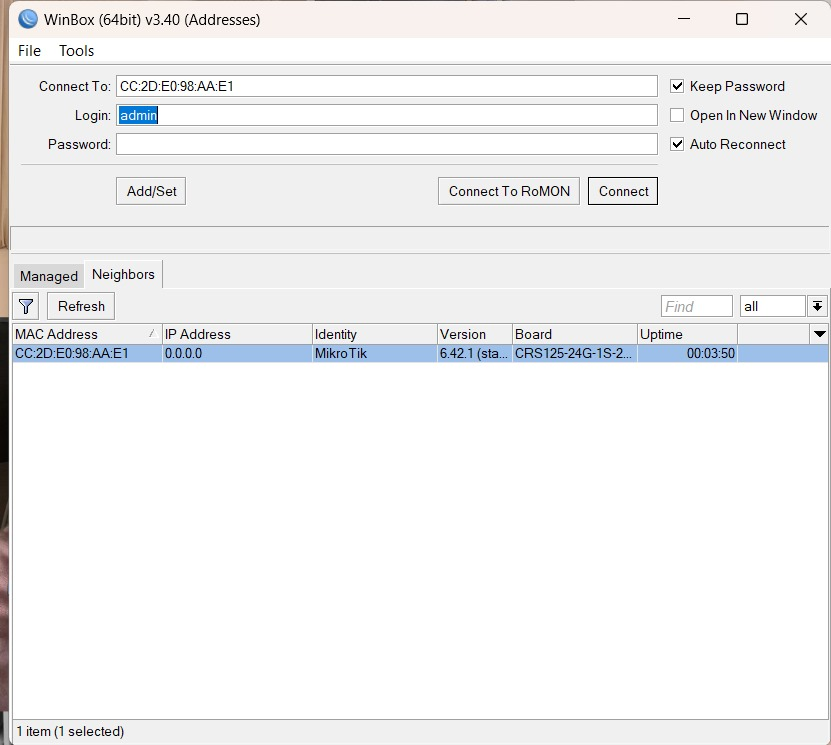
\includegraphics[width=0.5\linewidth]{P3/img/step1.jpg}
		\caption{Step 1}
		\label{fig:gambar1}
	\end{figure}

	% poin 2
	\item  Jadikan Router menjadi DHCP Client agar bisa mendapat IP address dari Internet ITS. IP >
	Klik DHCP Client > Tambahkan DHCP Client > Pilih interface yang terhubung dengan Internet
	(ether6)> Klik Apply > Klik OK.
	\begin{figure}[H]
		\centering
		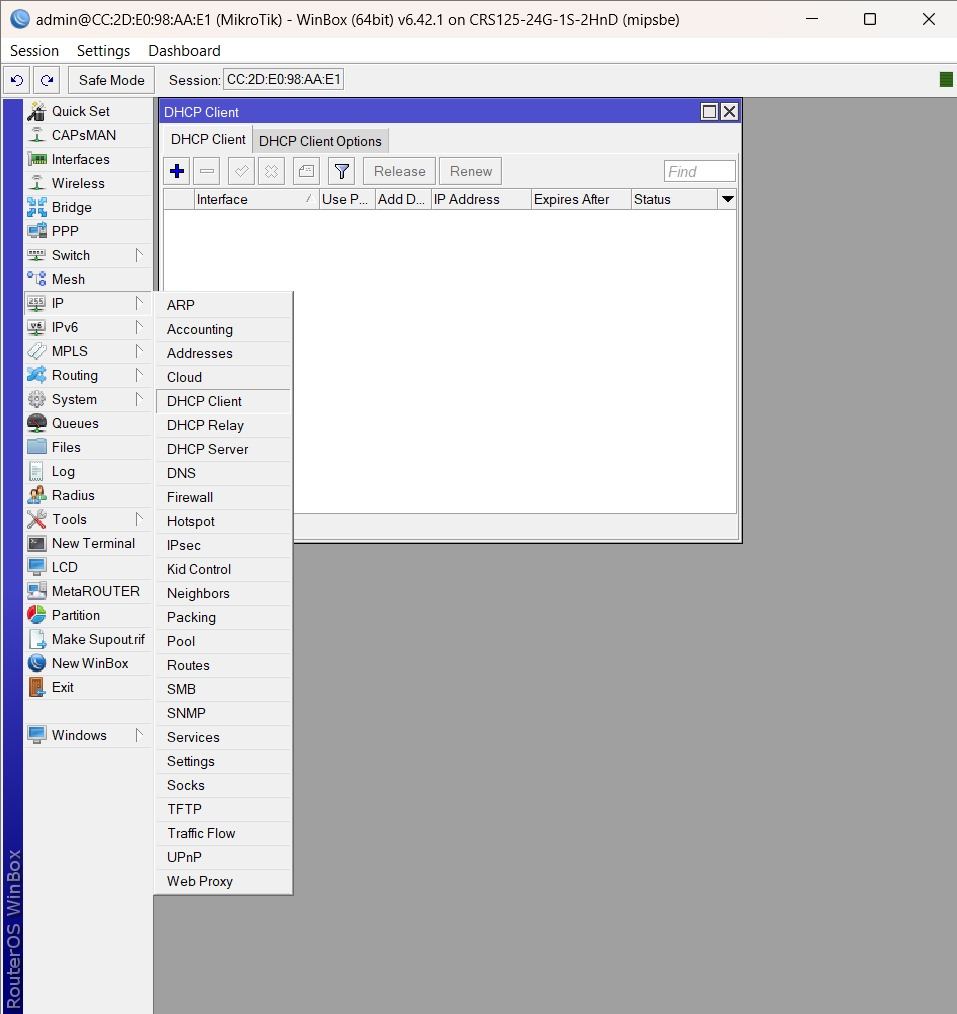
\includegraphics[width=0.5\linewidth]{P3/img/step2.jpg}
		\caption{Step 2.1}
		\label{fig:gambar2.1}

		\centering
		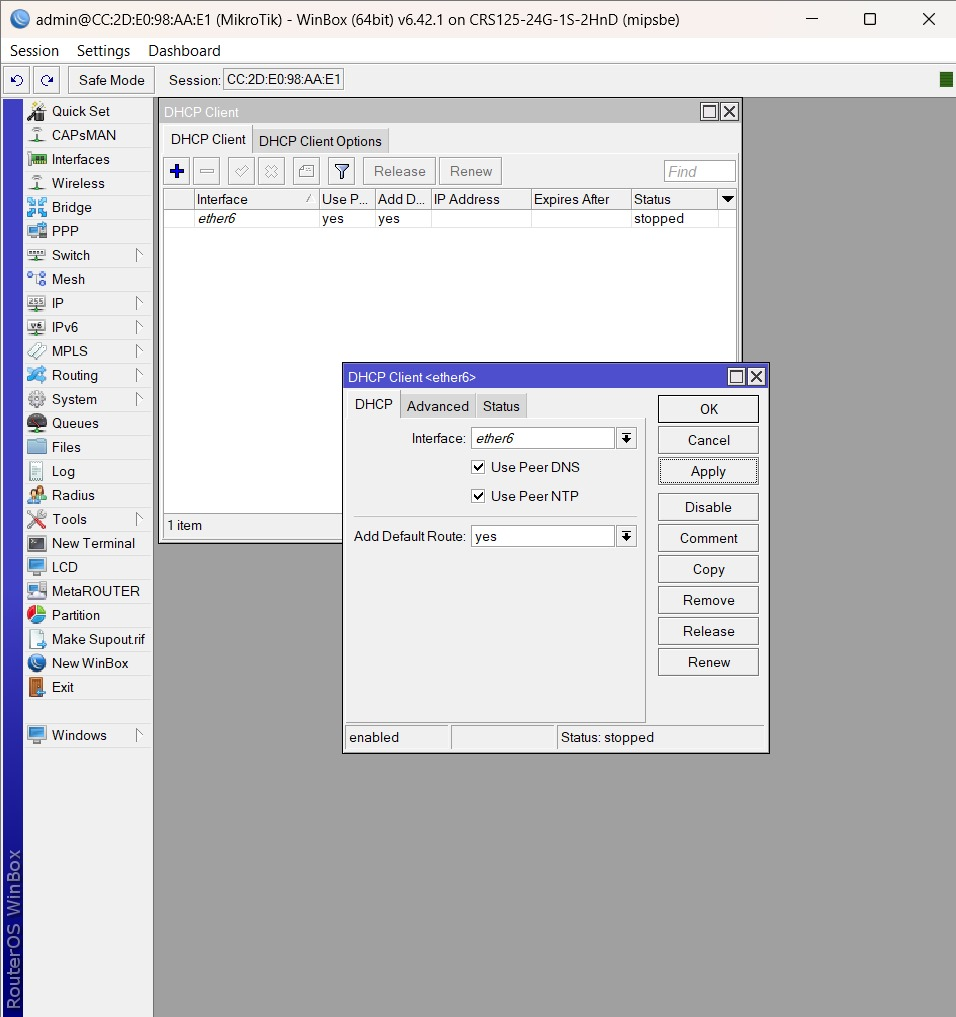
\includegraphics[width=0.5\linewidth]{P3/img/step2.2.jpg}
		\caption{Step 2.2}
		\label{fig:gambar2.2}
	\end{figure}

	% poin 3
	\item Buat IP address pada Router yang menghubungkan PC dengan Router. Tambahkan IP address
	> Isi address > Pilih Interface yang terhubung ke PC (ether2) > Klik Apply > Klik OK.
	\begin{figure}[H]
		\centering
		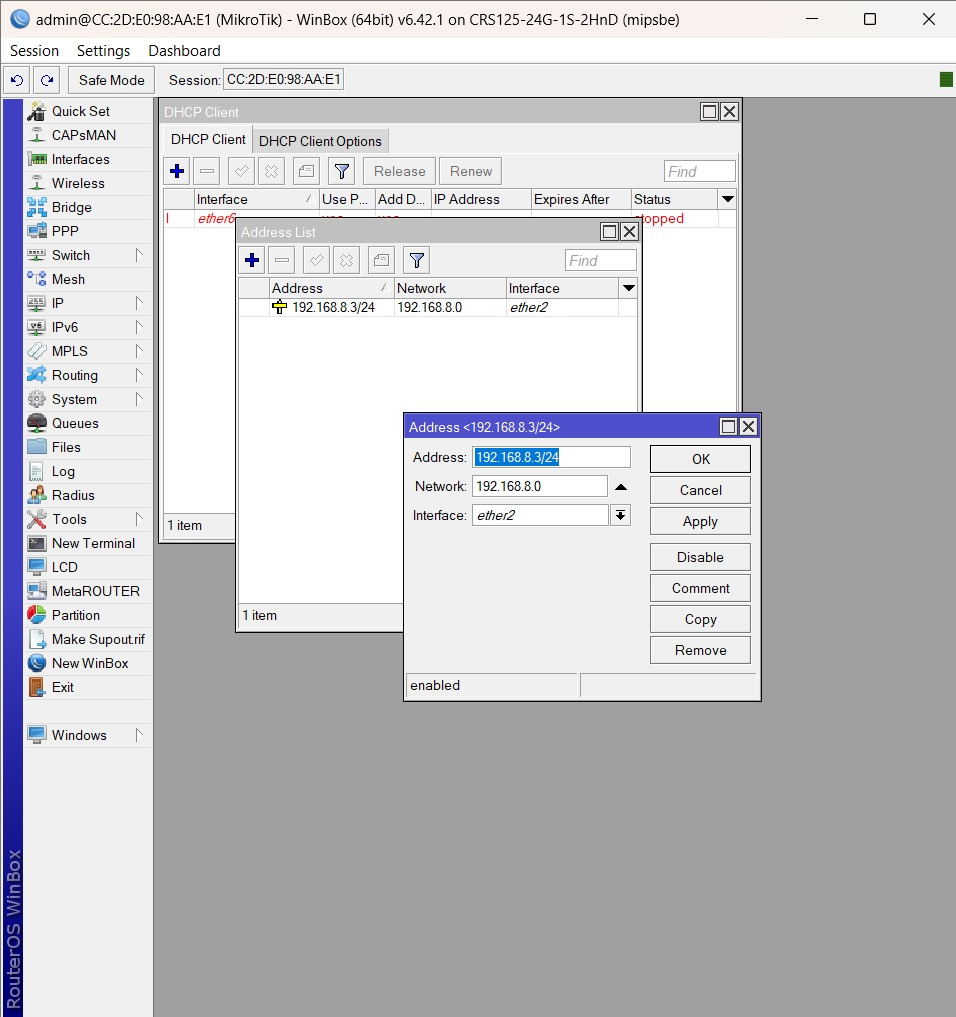
\includegraphics[width=0.5\linewidth]{P3/img/step3.jpg}
		\caption{Step 3}
		\label{fig:gambar3}
	\end{figure}

	% poin 4
	\item Jadikan Router menjadi DHCP Server agar bisa memberikan IP address secara DInamis kepada perangkat yang akan terhubung ke Router. IP > Klik DHCP Server
	\begin{figure}[H]
		\centering
		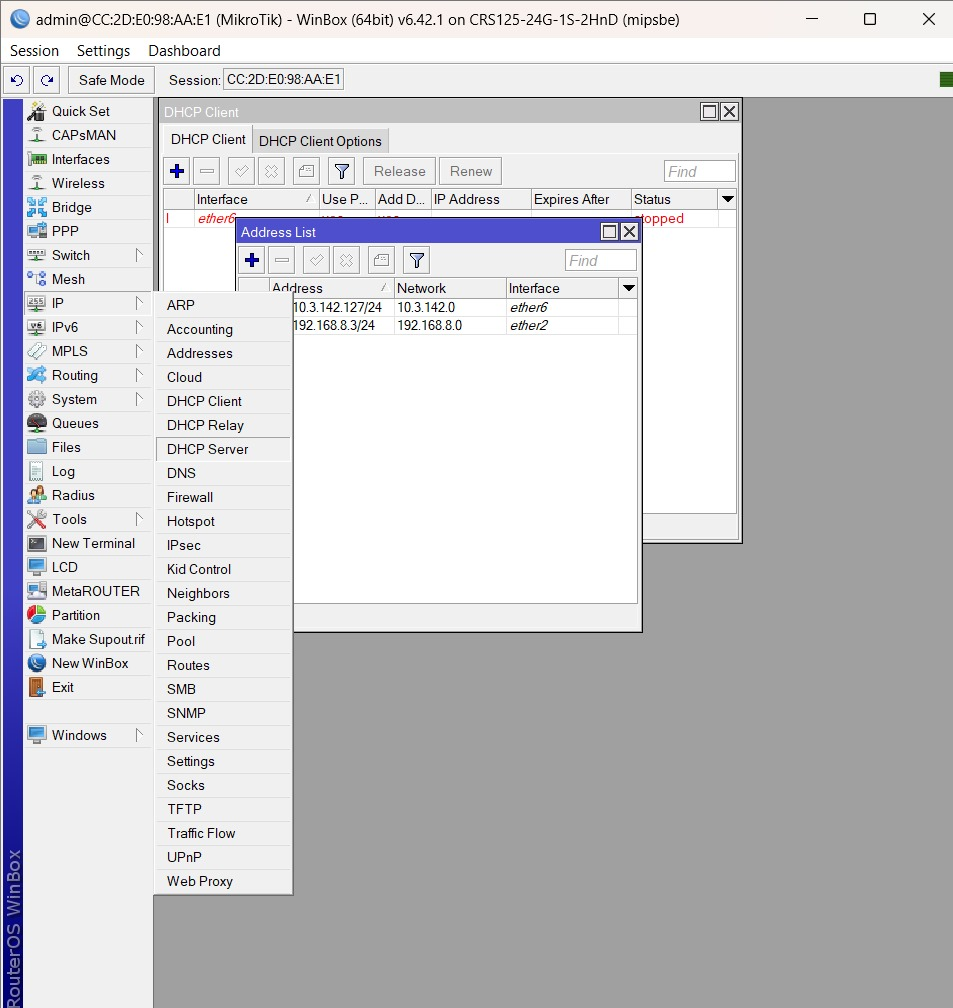
\includegraphics[width=0.5\linewidth]{P3/img/step4.jpg}
		\caption{Step 4}
		\label{fig:gambar4}
	\end{figure}

	% poin 5
	\item Untuk menjadikan Router menjadi DHCP Server ada beberapa parameter yang harus di buat.
	Parameter pertama adalah DHCP Server Interface yang akan menjadi port Output DHCP Server. Klik DHCP Setup > Pilih Interface yang yang akan menjadi Server (ether2).	
	\begin{figure}[H]
		\centering
		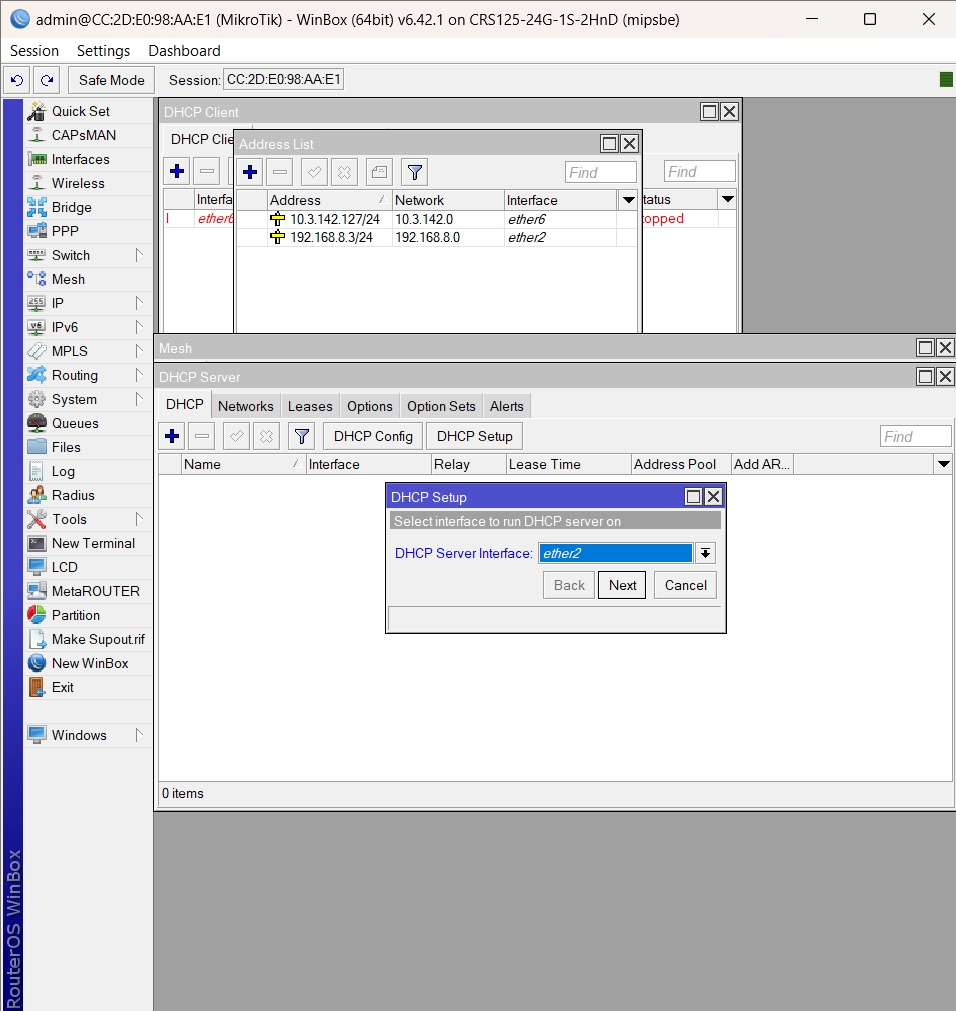
\includegraphics[width=0.5\linewidth]{P3/img/step5.jpg}
		\caption{Step 5}
		\label{fig:gambar4}
	\end{figure}

	% poin 6
	\item Parameter kedua adalah DHCP Address Space. Isinya adalah alamat Network yang ingin dibuat. Oleh karena itu alamat IP nya diakhiri dengan angka 0.
	\begin{figure}[H]
		\centering
		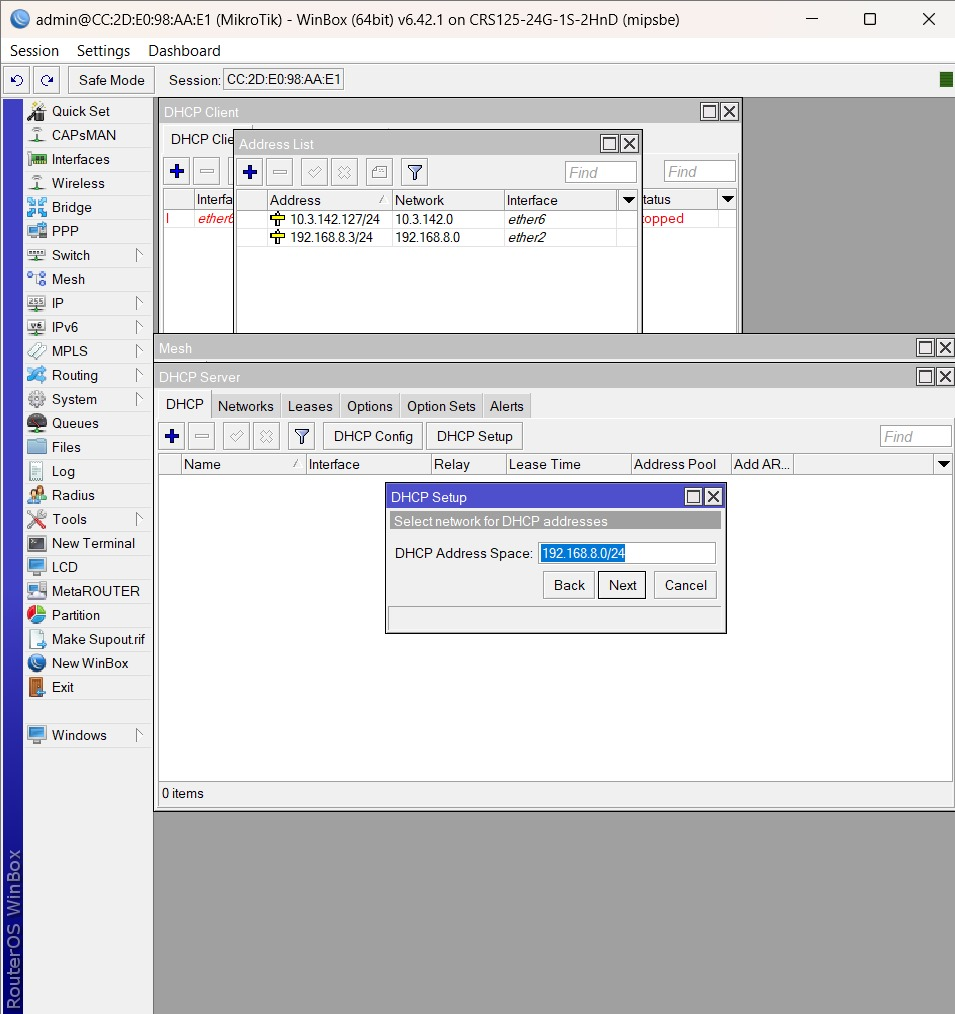
\includegraphics[width=0.5\linewidth]{P3/img/step6.jpg}
		\caption{Step 6}
		\label{fig:gambar4}
	\end{figure}

	% poin 7
	\item Parameter ketiga adalah Gateway for DHCP Network. Isinya adalah port pada Router yang
	akan menghubungkan Router dengan Network address yang sudah ditentukan.
	\begin{figure}[H]
		\centering
		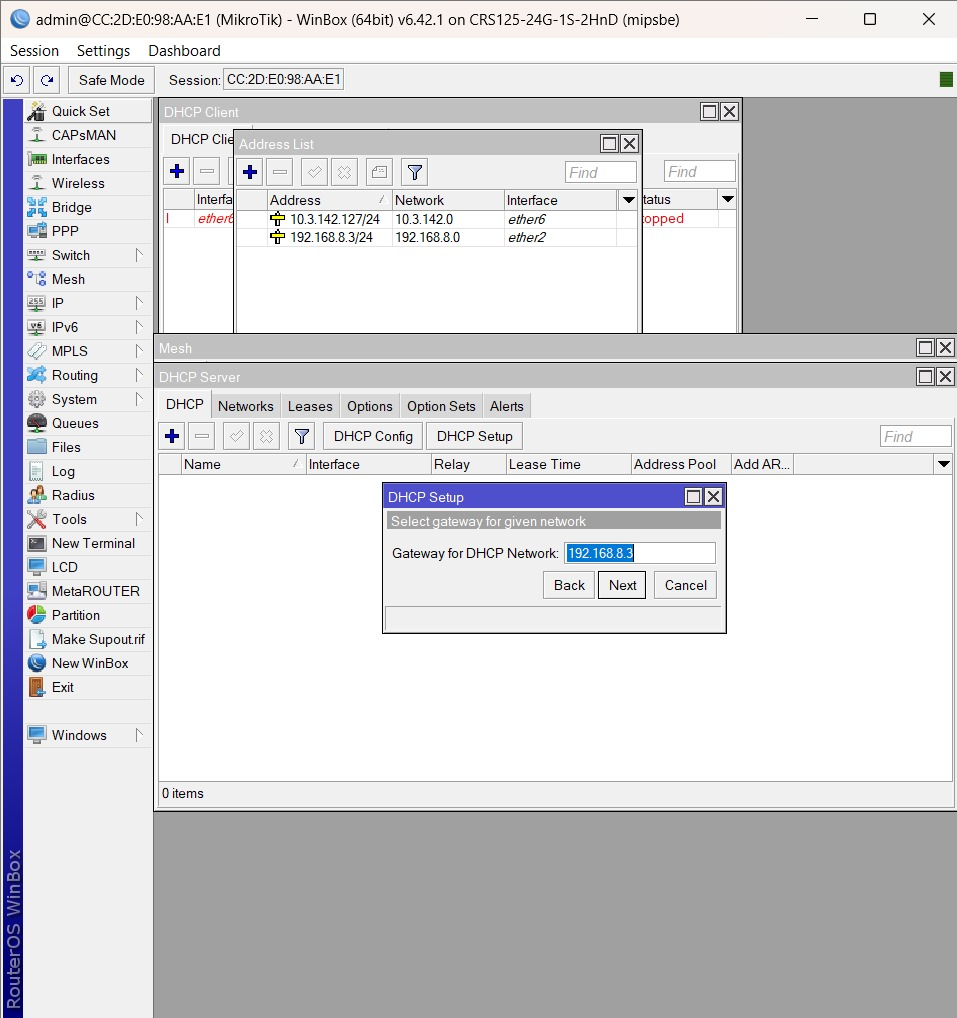
\includegraphics[width=0.5\linewidth]{P3/img/step7.jpg}
		\caption{Step 7}
		\label{fig:gambar4}
	\end{figure}

	% poin 8
	\item Parameter keempat adalah Adresses to Give Out. Isinya adalah range IP address yang akan
	diberikan kepada masing-masing perangkat yang akan terhubung. Pada Modul alamat yang
	dapat diberikan adalah antara 192.168.10.3 sampai 192.168.10.255.
	\begin{figure}[H]
		\centering
		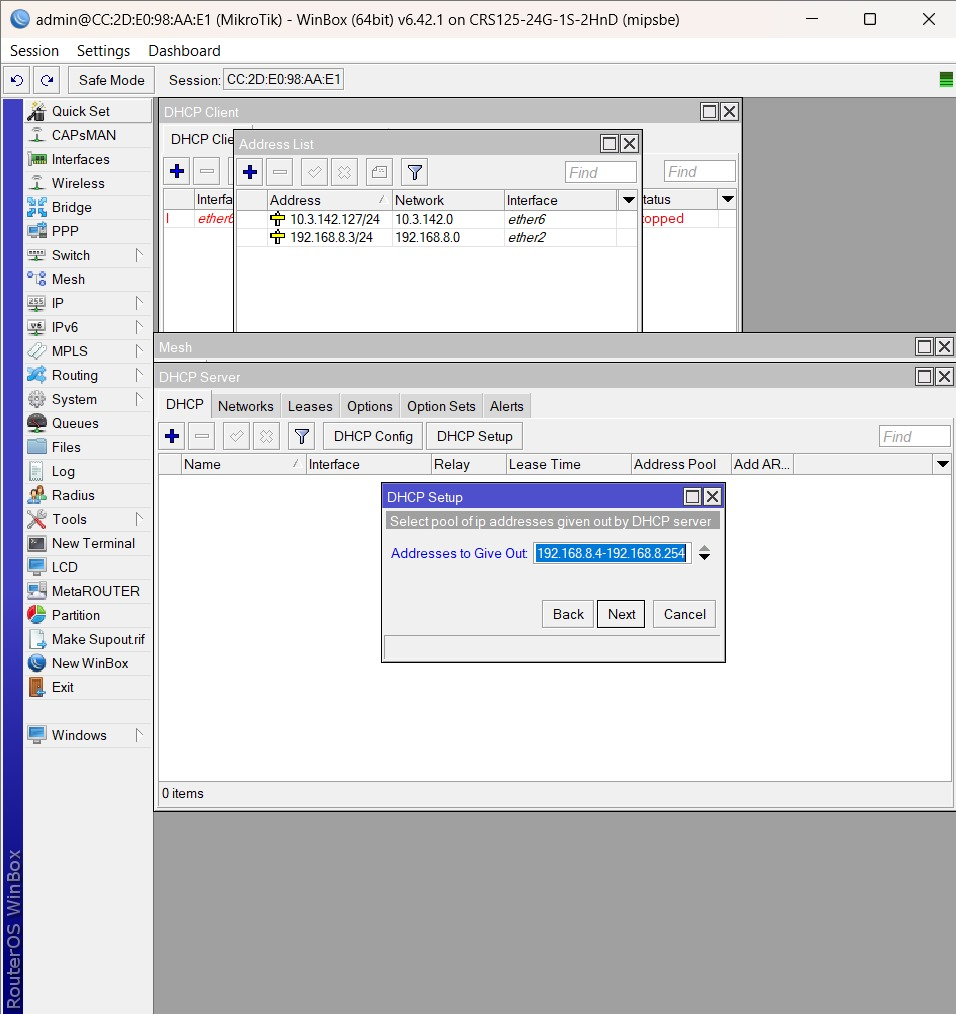
\includegraphics[width=0.5\linewidth]{P3/img/step8.jpg}
		\caption{Step 8}
		\label{fig:gambar4}
	\end{figure}

	% poin 9
	\item Parameter kelima adalah DNS Servers. Untuk opsi langsung saja Klik Next.
	\begin{figure}[H]
		\centering
		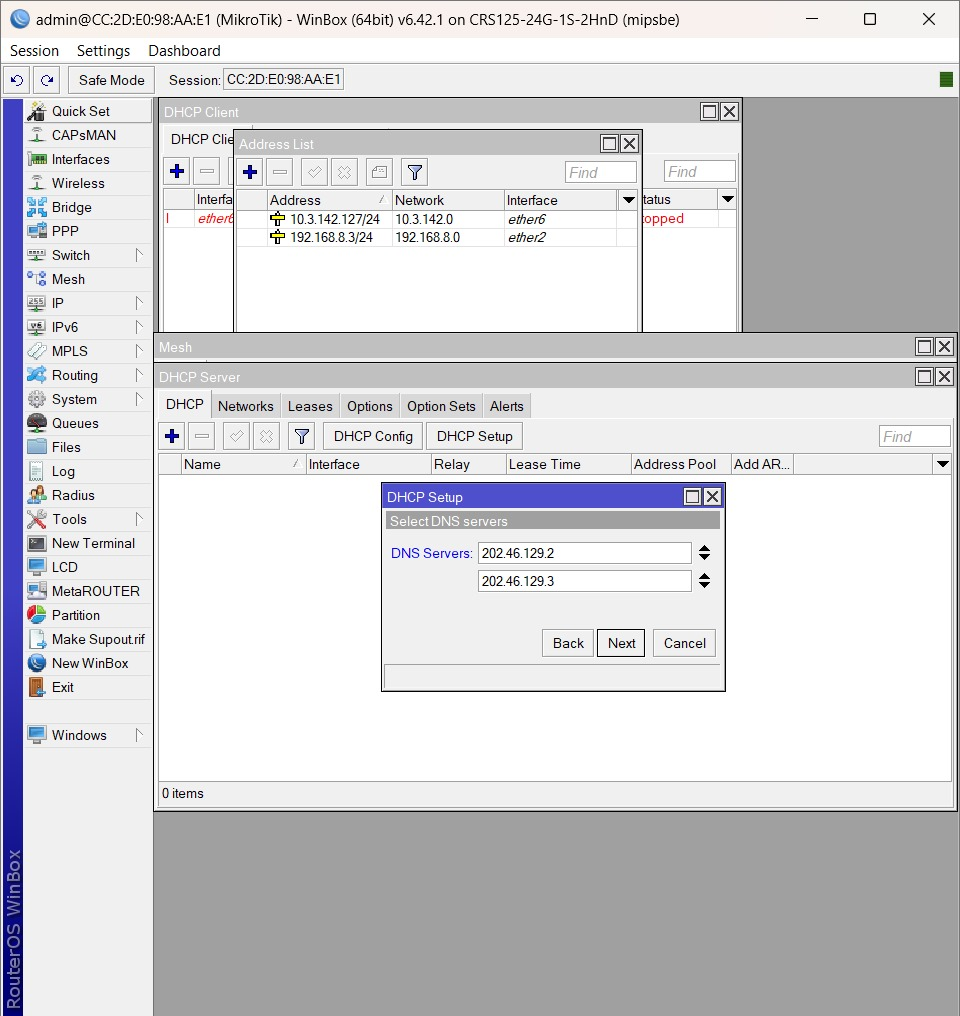
\includegraphics[width=0.5\linewidth]{P3/img/step9.jpg}
		\caption{Step 9}
		\label{fig:gambar4}
	\end{figure}

	% poin 10
	\item Parameter keenam adalah Lease Time. Lease Time dipakai untuk membatasi waktu penggunaan IP address yang diberikan oleh Router kepada Devices. Untuk opsi langsung saja Klik
	Next.
	\begin{figure}[H]
		\centering
		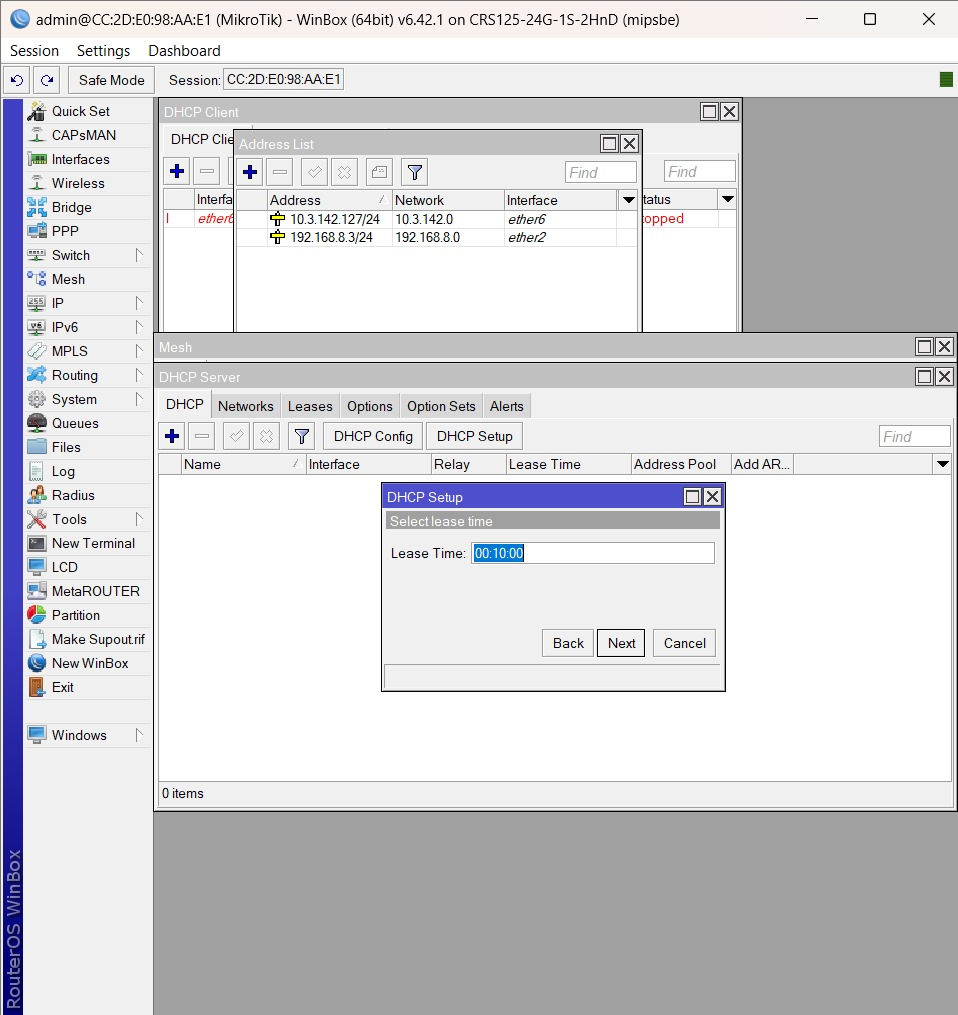
\includegraphics[width=0.5\linewidth]{P3/img/step10.jpg}
		\caption{Step 10}
		\label{fig:gambar4}
	\end{figure}

	% poin 11
	\item Pastikan IP Settings untuk koneksi Ethernet pada PC sudah pada Mode Automatic (DHCP).
	\begin{figure}[H]
		\centering
		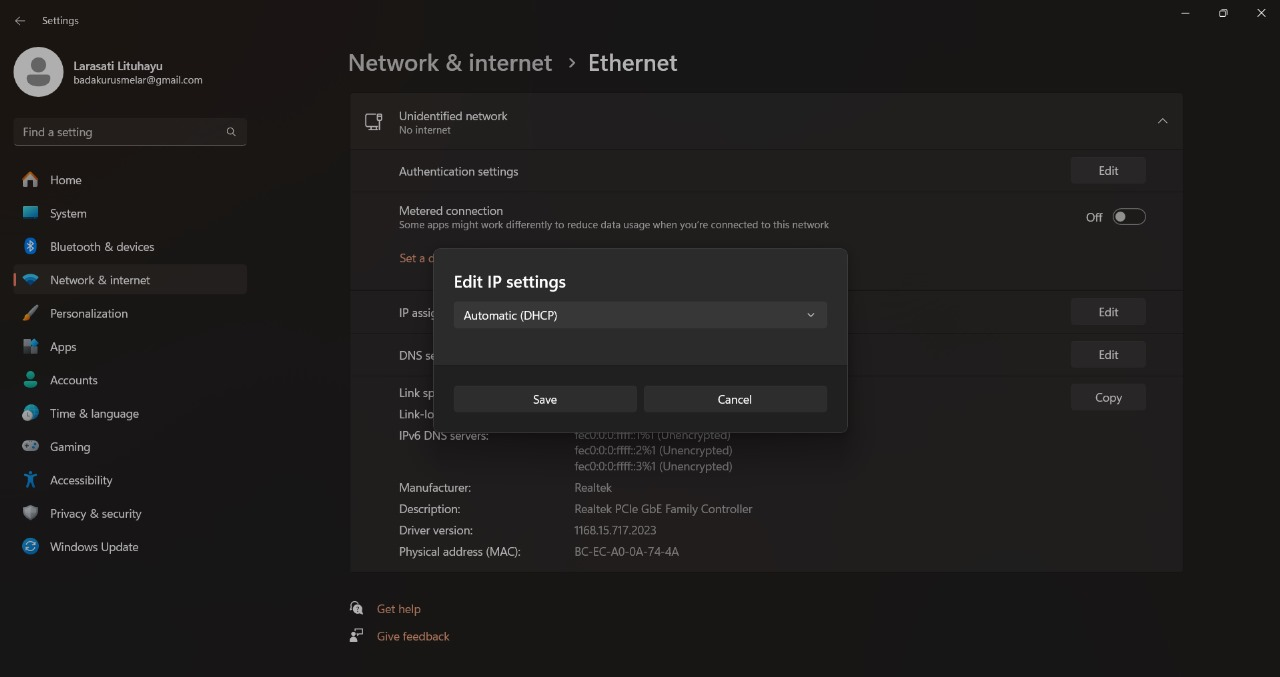
\includegraphics[width=0.5\linewidth]{P3/img/step11.jpg}
		\caption{Step 11}
		\label{fig:gambar4}
	\end{figure}

	% poin 12
	\item Agar PC yang berada pada jaringan lokal dapat terhubung ke jaringan publik, dapat digunakan
	layanan NAT (Network Address Translation) yang akan menerjemahkan IP lokal beserta port
	perangkat agar dapat terhubung dengan jaringan publik. IP > Klik Firewall.	
	\begin{figure}[H]
		\centering
		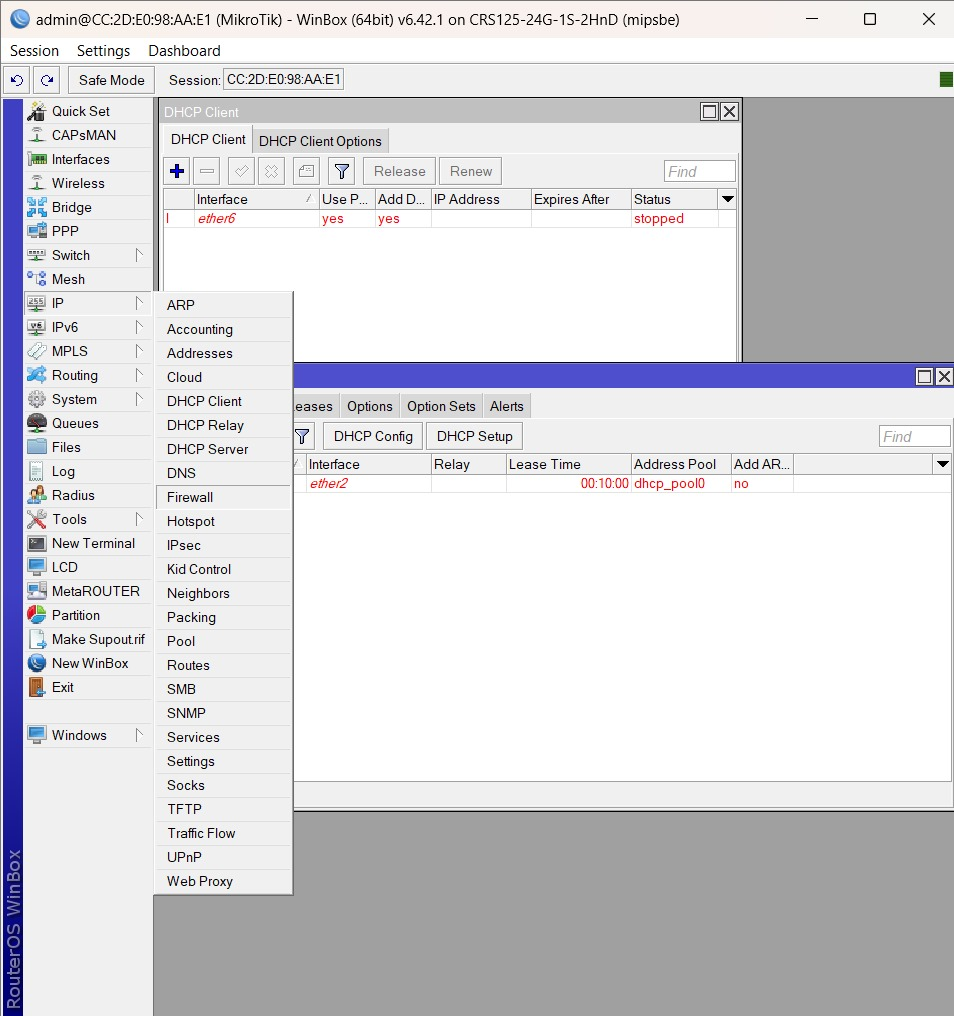
\includegraphics[width=0.5\linewidth]{P3/img/step12.jpg}
		\caption{Step 12}
		\label{fig:gambar4}
	\end{figure}

	% poin 13
	\item Buat NAT baru. Klik tab NAT > Tambahkan NAT > Pada Opsi Chain pilih srcnat > Pilih Out Interface yaitu port pada Router yang terhubung dengan Internet(ether6) > Klik Apply. Tambahkan
	Action pada tab Action. Pada Opsi Action pilih masquerade > Klik Apply > Klik OK.
	\begin{figure}[H]
		\centering
		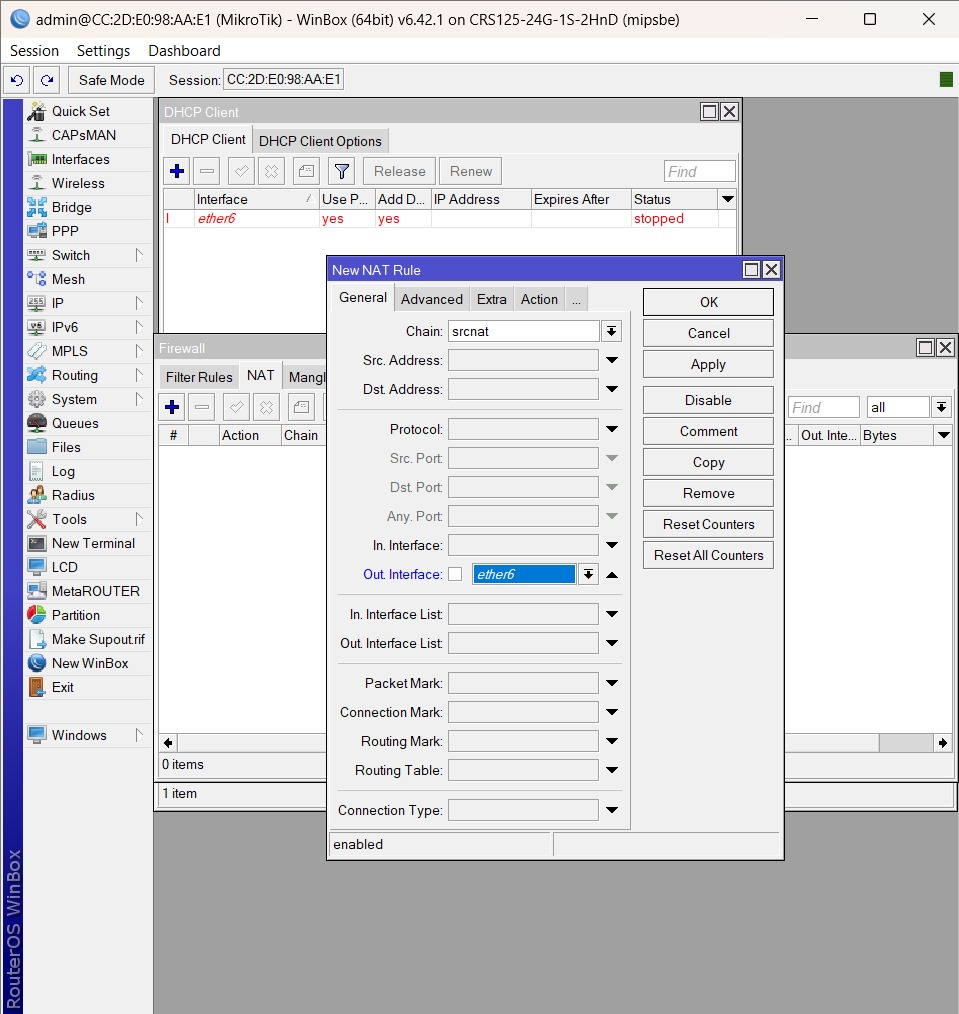
\includegraphics[width=0.5\linewidth]{P3/img/step13.1.jpg}
		\caption{Step 13.1}
		\label{fig:gambar4}

		\centering
		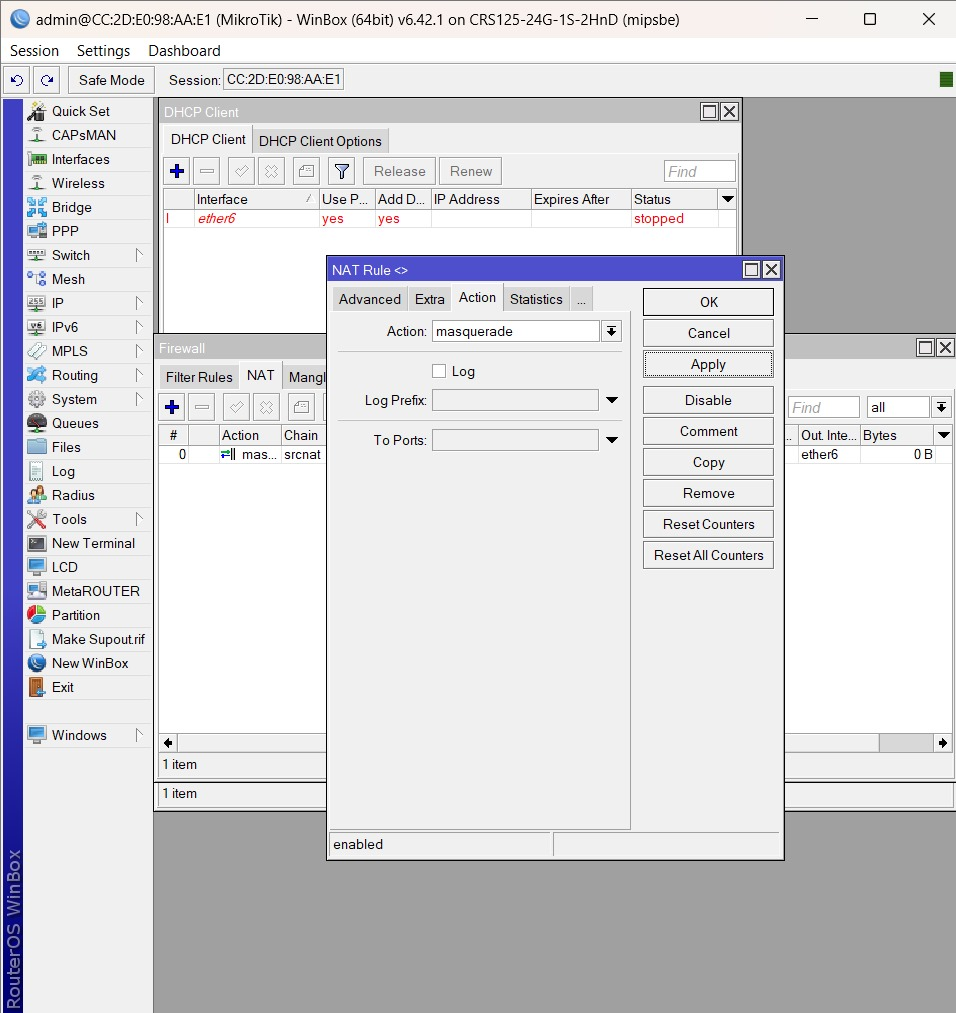
\includegraphics[width=0.5\linewidth]{P3/img/step13.2.jpg}
		\caption{Step 13.2}
		\label{fig:gambar4}
	\end{figure}

	% poin 14
	\item Lakukan test ping ke 8.8.8.8 untuk memastikan PC sudah terhubung dengan jaringan luar.
	\begin{figure}[H]
		\centering
		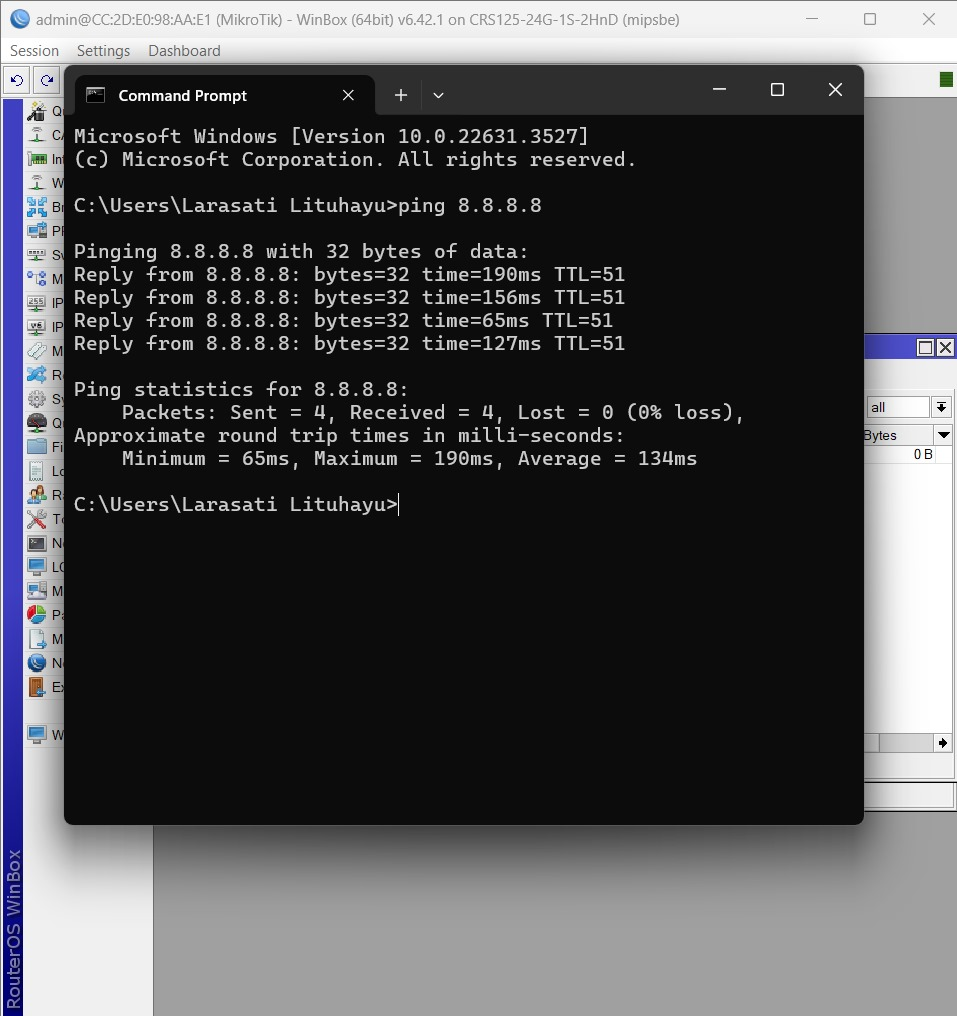
\includegraphics[width=0.5\linewidth]{P3/img/step14.jpg}
		\caption{Step 14}
		\label{fig:gambar4}
	\end{figure}

	% poin 15
	\item Lakukan test bandwidth menggunakan SPEEDTEST melalui search engine PC.
	\begin{figure}[H]
		\centering
		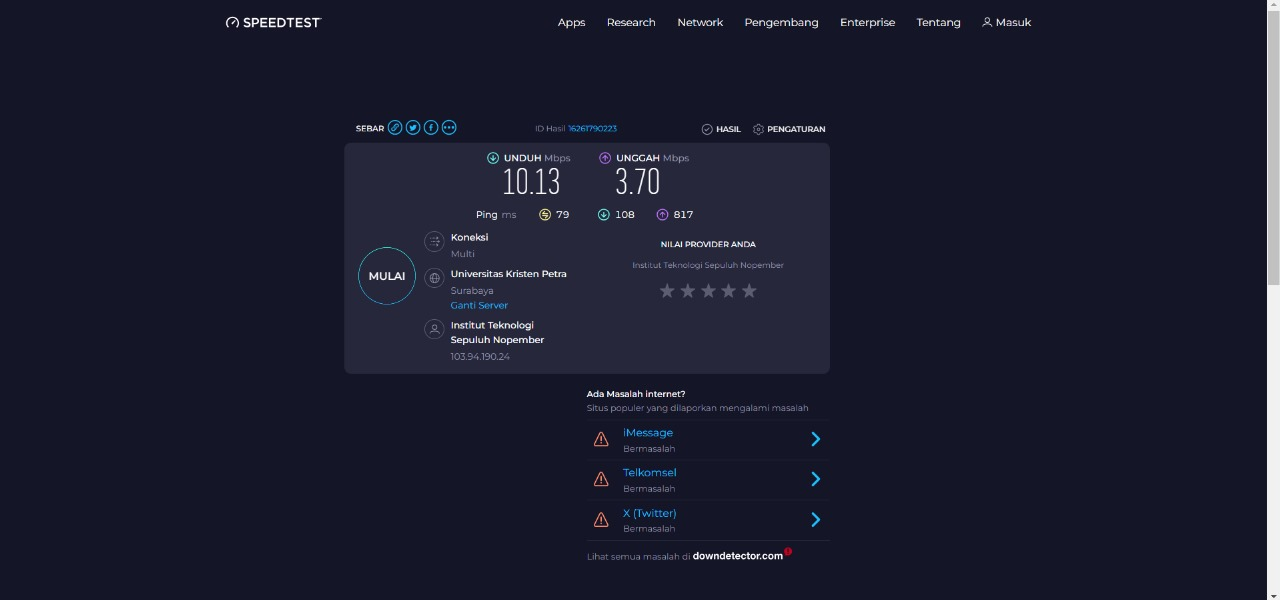
\includegraphics[width=0.5\linewidth]{P3/img/step15.jpg}
		\caption{Step 15}
		\label{fig:gambar4}
	\end{figure}

	% poin 16
	\item Lakukan pembatasan bandwidht menggunakan Queues. Klik Queues, Klik Queues > Tambahkan Queue List > Isi Nama perangkat yang ingin dibatasi bandwidthnya > Isi target dengan IP
	address PC (dapat dilihat melalui ipconfig) > Batasi Target Uploadnya menjadi 1M > Batasi Target Downloadnya menjadi 1M > Klik Apply > Klik OK.	
	\begin{figure}[H]
		\centering
		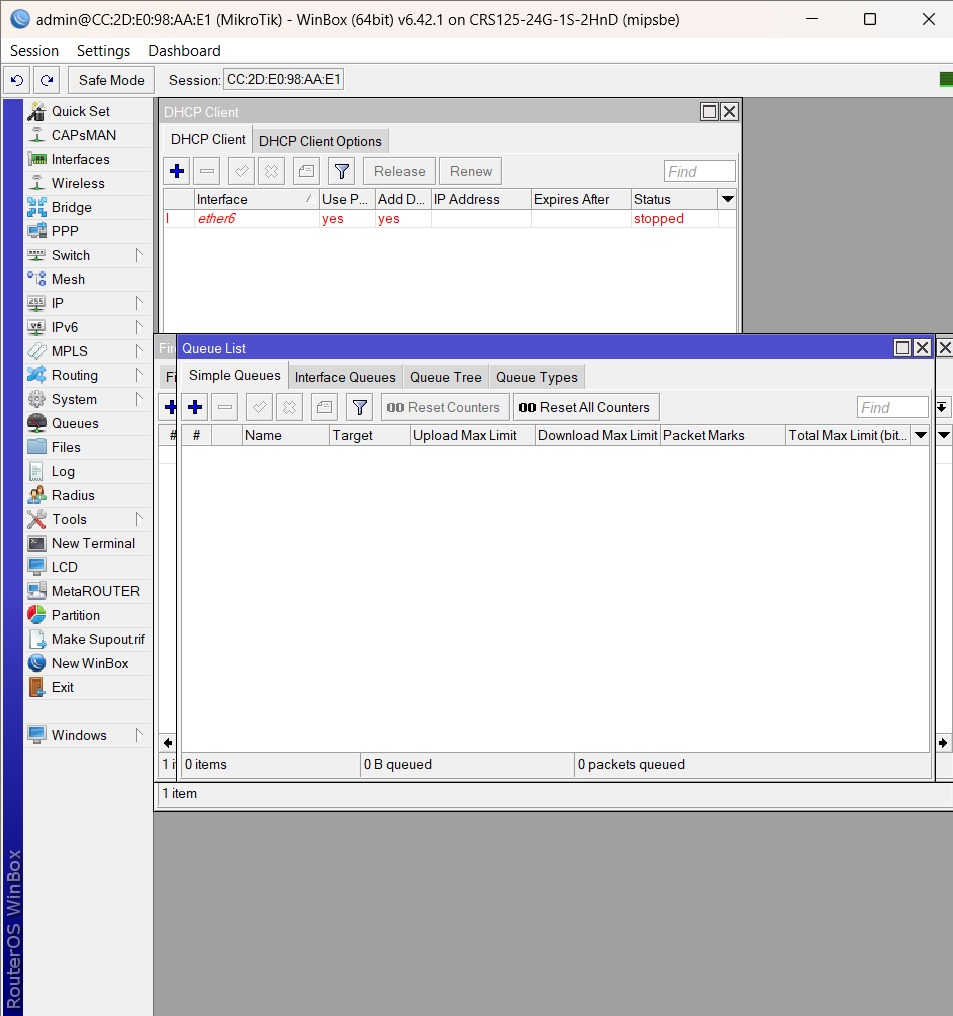
\includegraphics[width=0.5\linewidth]{P3/img/step16.jpg}
		\caption{Step 16.1}
		\label{fig:gambar4}

		\centering
		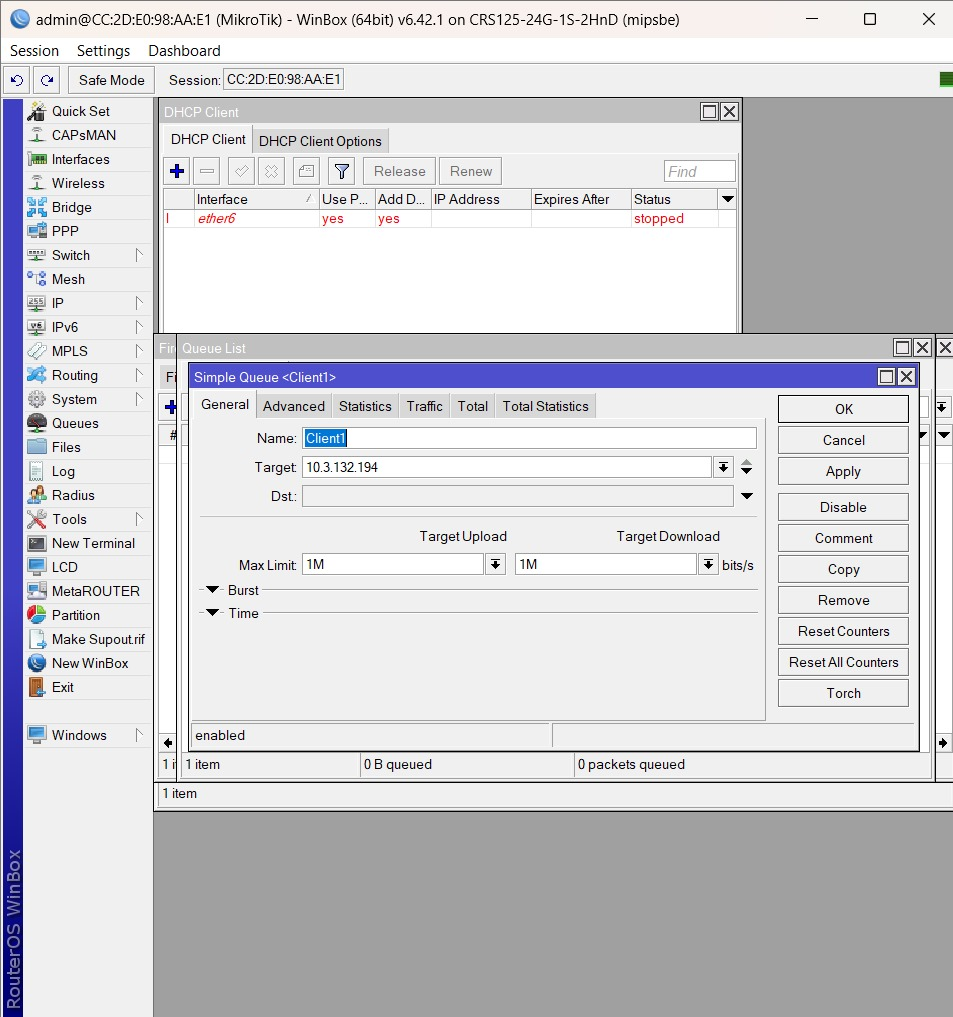
\includegraphics[width=0.5\linewidth]{P3/img/step16.2.jpg}
		\caption{Step 16.2}
		\label{fig:gambar4}
	\end{figure}

	% poin 17
	\item Lakukan test bandwidth kembali menggunakan SPEEDTEST melalui search engine PC.
	\begin{figure}[H]
		\centering
		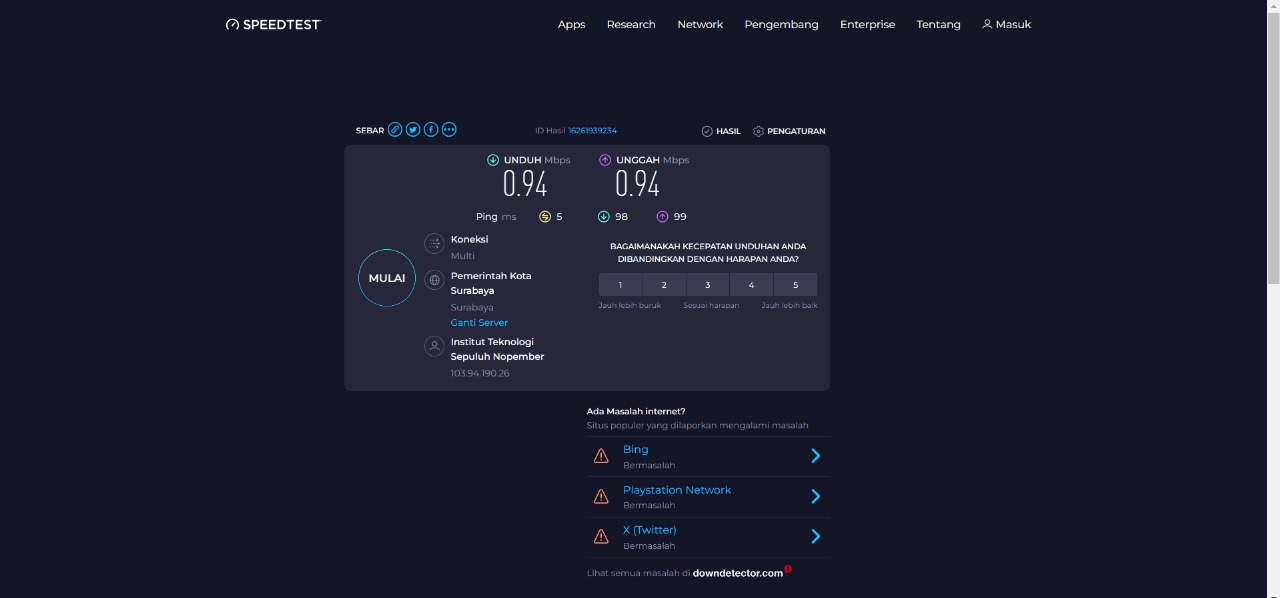
\includegraphics[width=0.5\linewidth]{P3/img/step17.jpg}
		\caption{Step 17}
		\label{fig:gambar4}
	\end{figure}

\end{enumerate}


\section{Hasil Percobaan}
Diisi nanti setelah praktikum
%===========================================================%

\section{Kesimpulan}
Diisi nanti setelah praktikum
%===========================================================%

\section{Lampiran}

\subsection{Tugas Pendahuluan}
\begin{enumerate}
	\item Apa yang dimaksud dengan Simple Queue? \\
	\\ \indent Simple Queue adalah metode bandwidth management yang tersedia di RouterOS Mikrotik. 
	Metode ini memanfaatkan Memory/RAM di router sebagai buffer penampungan antrian paket data. 
	Jika antrian paket data sudah memenuhi penampungan maka paket data yang tidak tertampung akan di Drop. 
	Jika protocolnya TCP, paket yang di drop akan dikirim ulang oleh server. 
	\\ \\ \indent Simple Queue memiliki parameter dasar seperti Target dan Max-limit, yang digunakan untuk memberikan batas maksimal bandwidth untuk si target. 
	Target dapat berupa IP address, network address, dan bisa juga interface yang akan diatur bandwidthnya. Max-limit Upload atau Download digunakan untuk memberikan batas maksimal bandwidth untuk si target. 
	Simple Queue mampu melimit Upload dan download secara terpisah atau Total (Upload+download) sekaligus dalam satu rule menggunakan tab Total. 
	Setiap rule pada Simple Queue dapat berdiri sendiri ataupun dapat juga disusun dalam sebuah hierarki dengan mengarahkan Parent ke rule lain. 
	Parameter lain juga bisa dimanfaatkan untuk membuat rule semakin spesifik seperti Dst, Priority, Packete Mark dan sebagainya

	\item Keuntungan apa yang bisa didapat jika diterapkan ke suatu network?
	\\ Keuntungan yang didapat jika menerapkan simple queue ke suatu network adalah : 
	\begin{itemize}
		\item[\ding{58}] Metode Simple Queues dinilai lebih sederhana dalam proses konfigurasinya, sehingga cenderung lebih mudah dan cepat diatur.
		\item[\ding{58}] Memungkinkan pemantauan penggunaan bandwidth, baik secara real-time dan historis, untuk kebutuhan analisis lebih lanjut.
		\item[\ding{58}] Memungkinkan pengaturan bandwidth secara spesifik untuk setiap client atau group client, sehingga dapat memastikan bahwa setiap client mendapatkan jatah bandwidth yang sesuai dengan kebutuhan mereka
		\item[\ding{58}] Memungkinkan pengaturan prioritas traffic yang masuk ke dalam jaringan, sehingga traffic yang lebih penting dapat dijamin mendapatkan kecepatan transfer yang lebih cepat 
	\end{itemize}

\end{enumerate}

\subsection{Dokumentasi saat Praktikum}
Diisi nanti setelah praktikum
\begin{figure}[H]
	\centering
	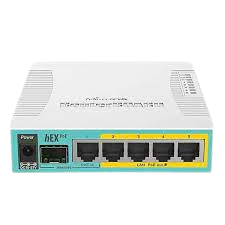
\includegraphics[width=0.75\linewidth]{P1/img/contoh.png}
	\caption{Dokumentasi saat praktikum}
	\label{fig:gambar32}
\end{figure}
\end{document}

